\documentclass[nooutcomes,noauthor,hints,handout]{ximera}

\graphicspath{  
{./}
{./whoAreYou/}
{./drawingWithTheTurtle/}
{./bisectionMethod/}
{./circles/}
{./anglesAndRightTriangles/}
{./lawOfSines/}
{./lawOfCosines/}
{./plotter/}
{./staircases/}
{./pitch/}
{./qualityControl/}
{./symmetry/}
{./nGonBlock/}
}


%% page layout
\usepackage[cm,headings]{fullpage}
\raggedright
\setlength\headheight{13.6pt}


%% fonts
\usepackage{euler}

\usepackage{FiraMono}
\renewcommand\familydefault{\ttdefault} 
\usepackage[defaultmathsizes]{mathastext}
\usepackage[htt]{hyphenat}

\usepackage[T1]{fontenc}
\usepackage[scaled=1]{FiraSans}

%\usepackage{wedn}
\usepackage{pbsi} %% Answer font


\usepackage{cancel} %% strike through in pitch/pitch.tex


%% \usepackage{ulem} %% 
%% \renewcommand{\ULthickness}{2pt}% changes underline thickness

\tikzset{>=stealth}

\usepackage{adjustbox}

\setcounter{titlenumber}{-1}

%% journal style
\makeatletter
\newcommand\journalstyle{%
  \def\activitystyle{activity-chapter}
  \def\maketitle{%
    \addtocounter{titlenumber}{1}%
                {\flushleft\small\sffamily\bfseries\@pretitle\par\vspace{-1.5em}}%
                {\flushleft\LARGE\sffamily\bfseries\thetitlenumber\hspace{1em}\@title \par }%
                {\vskip .6em\noindent\textit\theabstract\setcounter{question}{0}\setcounter{sectiontitlenumber}{0}}%
                    \par\vspace{2em}
                    \phantomsection\addcontentsline{toc}{section}{\thetitlenumber\hspace{1em}\textbf{\@title}}%
                     }}
\makeatother



%% thm like environments
\let\question\relax
\let\endquestion\relax

\newtheoremstyle{QuestionStyle}{\topsep}{\topsep}%%% space between body and thm
		{}                      %%% Thm body font
		{}                              %%% Indent amount (empty = no indent)
		{\bfseries}            %%% Thm head font
		{)}                              %%% Punctuation after thm head
		{ }                           %%% Space after thm head
		{\thmnumber{#2}\thmnote{ \bfseries(#3)}}%%% Thm head spec
\theoremstyle{QuestionStyle}
\newtheorem{question}{}



\let\freeResponse\relax
\let\endfreeResponse\relax

%% \newtheoremstyle{ResponseStyle}{\topsep}{\topsep}%%% space between body and thm
%% 		{\wedn\bfseries}                      %%% Thm body font
%% 		{}                              %%% Indent amount (empty = no indent)
%% 		{\wedn\bfseries}            %%% Thm head font
%% 		{}                              %%% Punctuation after thm head
%% 		{3ex}                           %%% Space after thm head
%% 		{\underline{\underline{\thmname{#1}}}}%%% Thm head spec
%% \theoremstyle{ResponseStyle}

\usepackage[tikz]{mdframed}
\mdfdefinestyle{ResponseStyle}{leftmargin=1cm,linecolor=black,roundcorner=5pt,
, font=\bsifamily,}%font=\wedn\bfseries\upshape,}


\ifhandout
\NewEnviron{freeResponse}{}
\else
%\newtheorem{freeResponse}{Response:}
\newenvironment{freeResponse}{\begin{mdframed}[style=ResponseStyle]}{\end{mdframed}}
\fi



%% attempting to automate outcomes.

%% \newwrite\outcomefile
%%   \immediate\openout\outcomefile=\jobname.oc
%% \renewcommand{\outcome}[1]{\edef\theoutcomes{\theoutcomes #1~}%
%% \immediate\write\outcomefile{\unexpanded{\outcome}{#1}}}

%% \newcommand{\outcomelist}{\begin{itemize}\theoutcomes\end{itemize}}

%% \NewEnviron{listOutcomes}{\small\sffamily
%% After answering the following questions, students should be able to:
%% \begin{itemize}
%% \BODY
%% \end{itemize}
%% }
\usepackage[tikz]{mdframed}
\mdfdefinestyle{OutcomeStyle}{leftmargin=2cm,rightmargin=2cm,linecolor=black,roundcorner=5pt,
, font=\small\sffamily,}%font=\wedn\bfseries\upshape,}
\newenvironment{listOutcomes}{\begin{mdframed}[style=OutcomeStyle]After answering the following questions, students should be able to:\begin{itemize}}{\end{itemize}\end{mdframed}}



%% my commands

\newcommand{\snap}{{\bfseries\itshape\textsf{Snap!}}}
\newcommand{\flavor}{\link[\snap]{https://snap.berkeley.edu/}}
\newcommand{\mooculus}{\textsf{\textbf{MOOC}\textnormal{\textsf{ULUS}}}}


\usepackage{tkz-euclide}
\tikzstyle geometryDiagrams=[rounded corners=.5pt,ultra thick,color=black]
\colorlet{penColor}{black} % Color of a curve in a plot



\ifhandout\newcommand{\mynewpage}{\newpage}\else\newcommand{\mynewpage}{}\fi

\title{Let's apply ourselves}
%\SetWatermarkLightness{1}

\author{Bart Snapp}

\begin{document}
\begin{abstract}
  Let's apply what we know to solve problems!
\end{abstract}
\maketitle


\begin{listOutcomes}
\item Explain how shapes of the same area can have drastically
  different perimeters.
\item Apply concepts related to loci of points.
\item Draw perpendicular lines.
\item Use facts about the foci of ellipses to solve problems.    
\item Recognize that circles are determined by three points.
\item Translate classroom mathematics into real world mathematics. 
\item Critique and dismantle reasonable hypotheses in regard to geometry and arithmetic.
\end{listOutcomes}


\mynewpage



\begin{question}
  Recall that from some previous life you learned that a triangle of a
  given (fixed) area could have an ARBITRARILY LARGE perimeter.
  \begin{enumerate}
  \item Reproduce an argument that a triangle of a given (fixed) area
    could have an ARBITRARILY LARGE perimeter.
  \item \textit{Geometry Giorgio} claims it is obvious that of all the
    triangles with a fixed area and fixed height, an isosceles triangle
    has least perimeter, \textbf{since we can produce a triangle of the same height
      of arbitrarily large perimeter.} Is he correct?
  \item Imagine a triangle with two points that are fixed, and a third
    that can MOVE, provided that the PERIMETER of the triangle is
    fixed. \textbf{What is the locus of points determined by the the third
    point?} USE the shape of this locus to EXPLAIN WHY of all the
    triangles with a fixed area and fixed height, an isosceles triangle
    has least perimeter.
  \end{enumerate}
  \begin{freeResponse}
    \begin{enumerate}
    \item Consider this picture:
      \begin{center}
        \begin{tikzpicture}[geometryDiagrams]
          \coordinate (A) at (0,0);
          \coordinate (B) at (2,0);
          \coordinate (C) at (.5,3);
          \draw[pattern=horizontal lines] (A)--(B)--(C)--cycle;
          
          \draw[line width=5pt, ->] (2,1.5)--(4,1.5);
          
          \coordinate (AA) at (4,0);
          \coordinate (BB) at (6,0);
          \coordinate (CC) at (11,3);
          \draw[pattern=horizontal lines] (AA)--(BB)--(CC)--cycle;
          %% \tkzLabelSegment[right](BB,CC){$h$}
          %% \tkzLabelSegment[below](BB,AA){$b$}
          %% \tkzLabelSegment[below](B,A){$b$}


          \draw[thin,dashed] (-1,0)--(12,0);
          \draw[thin,dashed] (-1,3)--(12,3);
        \end{tikzpicture}
      \end{center}
      The triangle on the right has the same area as the triangle on
      the left. However, the perimeter of the triangle on the right is
      MUCH greater.  To obtain an arbitrarily large perimeter, simply
      shear the triangle more---by Cavalieri's principle the area will
      be unchanged.
    \item \textit{Geometry Giorgio's} conclusion may be correct, but his
      reasoning is not. 
      \begin{center}
        \begin{tikzpicture}[geometryDiagrams]
          \coordinate (A) at (0,0);
          \coordinate (B) at (2,0);
          \coordinate (C) at (1,3);
          \draw[pattern=horizontal lines] (A)--(B)--(C)--cycle;
          
          \draw[line width=5pt, ->] (3,1.5)--(5,1.5);
          
          \coordinate (AA) at (6,0);
          \coordinate (BB) at (8,0);
          \coordinate (CC) at (8,3);
          \draw[pattern=horizontal lines] (AA)--(BB)--(CC)--cycle;
          %% \tkzLabelSegment[right](BB,CC){$h$}
          %% \tkzLabelSegment[below](BB,AA){$b$}
          %% \tkzLabelSegment[below](B,A){$b$}


          \draw[thin,dashed] (-1,0)--(9,0);
          \draw[thin,dashed] (-1,3)--(9,3);
        \end{tikzpicture}
      \end{center}
      Shearing as above, we see that while one side gets longer, the
      other side gets shorter. We CANNOT directly SEE that the
      isosceles triangle has the least perimeter for a given area.
    \item So let's think about this. Given two points, if we want to
      make a triangle with a fixed perimeter, we need to think about
      all points so that the distance from the point to our given two
      points is constant. WAIT A SECOND---THAT'S AN ELLIPSE!
      \begin{center}
        \begin{tikzpicture}[geometryDiagrams]
          \coordinate (A) at (0,0);
          \coordinate (B) at (2,0);
          \coordinate (C) at (1,3);
          \draw[pattern=horizontal lines] (A)--(B)--(C)--cycle;
          
          \filldraw[black] (0,0) circle (2pt);
          \filldraw[black] (2,0) circle (2pt);
          \begin{scope}
            \clip (-2.2,-.5) rectangle (4.2,3.2);
            \draw (1,0) ellipse (3.16 and 3);
          \end{scope}

          \draw[thin,dashed] (-4,0)--(6,0);
          \draw[thin,dashed] (-4,3)--(6,3);
        \end{tikzpicture}
      \end{center}
      If the vertex of a triangle is on this ellipse, then the
      perimeter is as small as possible.  If we shear the triangle at
      all, the vertex will leave the ellipse, and hence the triangle
      will have a greater perimeter.
    \end{enumerate}
  \end{freeResponse}
  \end{question}
\mynewpage













\begin{question}
  In 1973, FedEx was a small company. They had a very clever idea:
  Find a city equidistant (by plane) from the cities they want to
  deliver to.  Make this ``central'' city a ``hub'' and ship
  everything there.  You don't have to take my word for it though,
  check out \link[what FedEx has to say about
    this]{https://www.fedex.com/en-us/about/policy/aviation/why-memphis.html}.
  The idea was very successful, and and now a standard practice in the
  industry.

  In general, solving a problem like this depends on a lot of
  factors. For us, it is enough to solve a much simpler problem. If we
  have three points forming a triangle, the point equidistant from the
  vertices is called the \textbf{circumcenter}. The circle that these
  points lie on is called the \textbf{circumcircle}.
  \begin{enumerate}
  \item EXPLAIN (in broad strokes) how to use a protractor, ruler, and
    compass to find the \textbf{circumcenter} and
    \textbf{circumcircle} of a triangle.
  \item For each of the following triangles , use a protractor, ruler,
    and compass (or an online tool like
    \link[\textsl{Geogebra}]{https://www.geogebra.org/classic}) to
    find the \textbf{circumcenter} and \textbf{circumcircle}.
    \begin{description}
    \item[This acute triangle:] \begin{center}
      \raisebox{-.4\height}{\begin{tikzpicture}[geometryDiagrams]
          \draw[white] (-2in,0in) -- (2in,0in);
          \draw (1in,0in) -- (-1in,0in) -- (0in,2in) -- (1in,0in) -- (-1in,0in);
          \filldraw[black] (1in,0in) circle (2pt) ;
          \filldraw[black] (-1in,0) circle (2pt) ;
          \filldraw[black] (0in,2in) circle (2pt) ;
        \end{tikzpicture}}
      \end{center}
        \item[This obtuse triangle:]
          \begin{center}
      \raisebox{-.4\height}{
        \begin{tikzpicture}[geometryDiagrams]
          \draw (2in,0in) -- (-2in,0in) -- (0in,1in) -- (2in,0in) -- (-2in,0in);
          \filldraw[black] (2in,0in) circle (2pt) ;
          \filldraw[black] (-2in,0) circle (2pt) ;
          \filldraw[black] (0in,1in) circle (2pt) ;
        \end{tikzpicture}} 
      \end{center}
        \item[This right triangle:]
          \begin{center}
            \raisebox{-.4\height}{
              \begin{tikzpicture}[geometryDiagrams]
                \draw (4in,0in) -- (0in,0in) -- (2.56in,1.92in) -- (4in,0in) -- (0in,0in);
                \filldraw[black] (0in,0in) circle (2pt) ;
                \filldraw[black] (2.56in,1.92in) circle (2pt) ;
                \filldraw[black] (4in,0in) circle (2pt) ;
            \end{tikzpicture}} 
          \end{center}
    \end{description}
  \end{enumerate}
  \begin{freeResponse}
    \begin{enumerate}
      \item To find the circumcenter of a triangle. You intersect the
        perpendicular bisectors of the sides of the triangle.

        To find the perpendicular bisectors, Use the ruler to find the
        midpoint of a side. Then use the protractor to make a right
        angle. Draw this line, it will be the perpendicular bisector
        of the side.


        Once you have the circumcenter, use a compass to draw a circle
        with that as its center, and any vertex of the triangle as a
        point on the circle.
      \item Behold! My answers:
        \begin{description}
          \item[This acute triangle:] \raisebox{-.4\height}{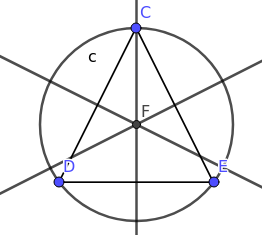
\includegraphics[width=.4\textwidth]{acuteCCSoln.png}}
          \item[This obtuse triangle:] \raisebox{-.4\height}{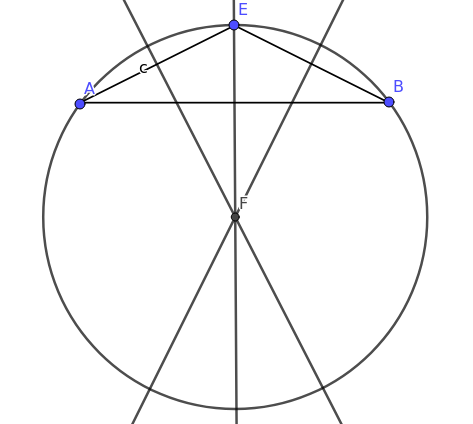
\includegraphics[width=.4\textwidth]{obtuseCCSoln.png}}
          \item[This right triangle:] \raisebox{-.4\height}{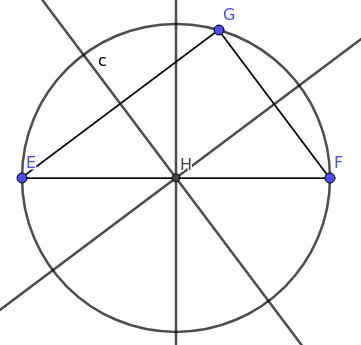
\includegraphics[width=.4\textwidth]{rightCCSoln.png}}
          \end{description}
    \end{enumerate}
  \end{freeResponse}
\end{question}
\mynewpage












\begin{question}
  On a cold morning in January of 1986, the Space Shuttle
  \textit{Challenger}'s solid rocket boosters suffered a malfunction,
  causing the primary fuel tank to explode shortly after lift-off.
  This resulted in the deaths of seven astronauts. 


  The \textit{Rogers Commission} was created to investigate the cause
  of the accident.  You can read (for yourself) a VERY ENLIGHTENING
  first hand account of this from Richard Feynman's book, \textit{What
    Do You Care What Other People Think?} In this book, we learn a lot
  about how NASA worked during the time of the Space Shuttle.

  \begin{enumerate}
  \item Find a picture of the Space Shuttle with its solid rocket
    boosters. \textbf{Clearly identify the solid rocket boosters on the photo.}
  \item In a typical launch, the solid rocket boosters fire for around
    $2$ minutes. Then they fall into the ocean and are recovered. Next
    they are shipped on large trucks back to the assembly
    building at NASA. \textbf{What do you think happens to the ``circular
    cross-section'' of the rocket boosters when all this happens?}
  \item NASA needed a way to detect if the solid rocket boosters were
    not round any more. Each rocket booster section has $180$ pins
    spaced evenly around the perimeter, where it connects to the next
    section. Here's a actual photo:
    \begin{center}%https://en.wikipedia.org/wiki/Space_Shuttle_Solid_Rocket_Booster#/media/File:STS-134_solid_rocket_booster_segment_stacking.jpg
      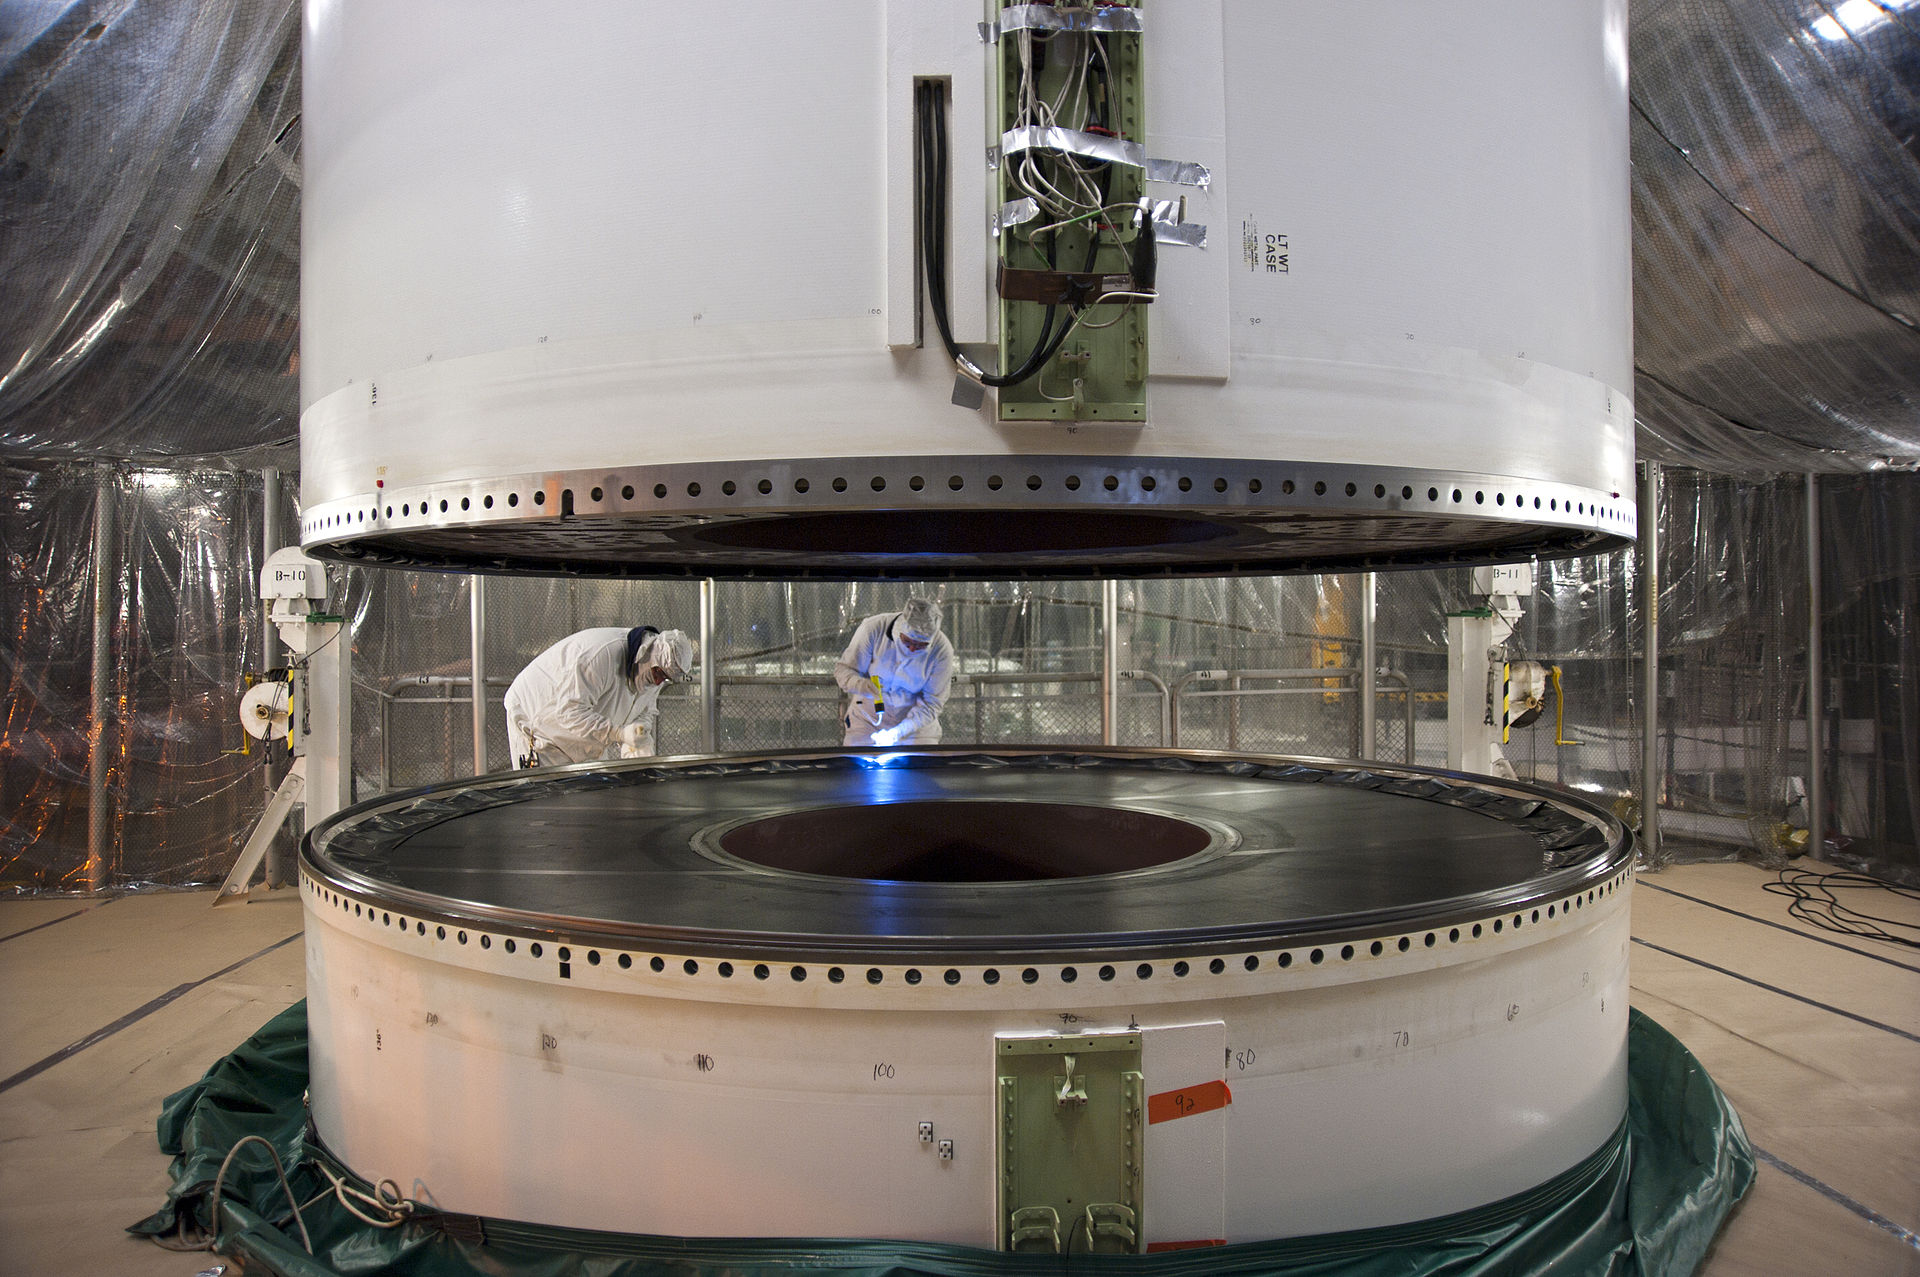
\includegraphics[width=.6\textwidth]{srbSections.jpg}
    \end{center}
    Apparently \textit{Geometry Giorgio} worked as a
    contractor for NASA. He suggested the following method to
    determine how ``circular'' the cross sections of the solid rocket
    booster were.
    
    \begin{quote}
      \textbf{\textit{Geometry Giorgio} says that to determine if the cross
        section is circular:}
      \begin{itemize}
      \item Define a DIAMETER to be the distance from one pin to a pin
        that is directly opposite the starting pin.
      \item Measure three diameters, separated by $60^\circ$.
      \item If these diameters agree, then the cross section is
        circular.
      \end{itemize}
    \end{quote}
    Try \textit{Geometry Giorgio}'s method on these THREE cross
    sections. Note, in real life you'd have $180$ pins to count. Here,
    I've only drawn $24$, this makes things easier to deal with.
    \begin{description}
    \item[This circle:] 
      \begin{center}
         \raisebox{-.4\height}{\begin{tikzpicture}[geometryDiagrams,scale=5]
          \draw [line cap=round,domain=0:360,black, line width=20pt,smooth] plot ({cos(\x)}, {sin(\x)} );
          \draw [line cap=round,domain=0:360,white, line width=18pt,smooth] plot ({cos(\x)}, {sin(\x)} );
          
          \foreach \x in {0,15,...,360}
                   {
                     \filldraw[black] ({cos(\x)}, {sin(\x)} ) circle (.2pt) ;
                   }
        \end{tikzpicture}}
      \end{center}
\item[This oval:] \begin{center}
   \raisebox{-.4\height}{\begin{tikzpicture}[geometryDiagrams,scale=5]
    \draw [line cap=round,domain=0:360,black, line width=20pt,smooth] plot ({(1+0.1*sin(\x))*sin(\x/2)}, {(1+0.1*sin(\x))*cos(\x/2)} );
    \draw [line cap=round,domain=0:360,black, line width=20pt,smooth] plot ({(1+0.1*sin(\x))*sin(\x/2+180)}, {(1+0.1*sin(\x))*cos(\x/2+180)} );
    
    \draw [line cap=round,domain=0:360,white, line width=18pt,smooth] plot ({(1+0.1*sin(\x))*sin(\x/2)}, {(1+0.1*sin(\x))*cos(\x/2)} );
    \draw [line cap=round,domain=0:360,white, line width=18pt,smooth] plot ({(1+0.1*sin(\x))*sin(\x/2+180)}, {(1+0.1*sin(\x))*cos(\x/2+180)} );
    
    \foreach \x in {0,30,...,360}
             {
               \filldraw[black] ({(1+0.1*sin(\x))*sin(\x/2)}, {(1+0.1*sin(\x))*cos(\x/2)} ) circle (.2pt) ;
               \filldraw[black] ({(1+0.1*sin(\x))*sin(\x/2+180)}, {(1+0.1*sin(\x))*cos(\x/2+180)} ) circle (.2pt) ;
             }
  \end{tikzpicture}}
\end{center}    
\item[This heart-shape:] \begin{center}
   \raisebox{-.4\height}{\begin{tikzpicture}[geometryDiagrams,scale=5]
    \draw [line cap=round,domain=0:360,black, line width=20pt,smooth] plot ({(1+0.1*sin(\x))*sin(\x/2)}, {(1+0.1*sin(\x))*cos(\x/2)} );
    \draw [line cap=round,domain=0:360,black, line width=20pt,smooth] plot ({(1-0.1*sin(\x))*sin(\x/2+180)}, {(1-0.1*sin(\x))*cos(\x/2+180)} );
    
    \draw [line cap=round,domain=0:360,white, line width=18pt,smooth] plot ({(1+0.1*sin(\x))*sin(\x/2)}, {(1+0.1*sin(\x))*cos(\x/2)} );
    \draw [line cap=round,domain=0:360,white, line width=18pt,smooth] plot ({(1-0.1*sin(\x))*sin(\x/2+180)}, {(1-0.1*sin(\x))*cos(\x/2+180)} );
    
    \foreach \x in {0,30,...,360}
             {
               \filldraw[black] ({(1+0.1*sin(\x))*sin(\x/2)}, {(1+0.1*sin(\x))*cos(\x/2)} ) circle (.2pt) ;
               \filldraw[black] ({(1-0.1*sin(\x))*sin(\x/2+180)}, {(1-0.1*sin(\x))*cos(\x/2+180)} ) circle (.2pt) ;
             }
  \end{tikzpicture}}
\end{center}
    \end{description}
\textbf{Is \textit{Geometry Giorgio's} claim correct? EXPLAIN how you
  arrived at your conclusion.}

\item PROPOSE an alternate method for detecting how ``circular'' the
  cross section of the solid rocket booster is. \textbf{Try your method on the THREE
    pictures above and discuss the results.}

  
  \end{enumerate}
  The cause of the \textit{Challenger's} explosion was directly
  related to the construction and tolerances of the solid rocket
  boosters. Eventually, two rubber O-rings that created the ``seal''
  between sections of the solid rocket booster were found to be the
  cause, as they did not function as desired in cold weather.


  This author finds it interesting that in the aftermath of the
  \textit{Challenger} disaster, the solid rocket boosters were
  redesigned to fit together better, a third O-ring was added, and
  \textbf{cold-weather launches were aborted.}


  \begin{freeResponse}
    \begin{enumerate}
    \item Here is a picture of the Space Shuttle with its solid rocket boosters:
      \begin{center}
        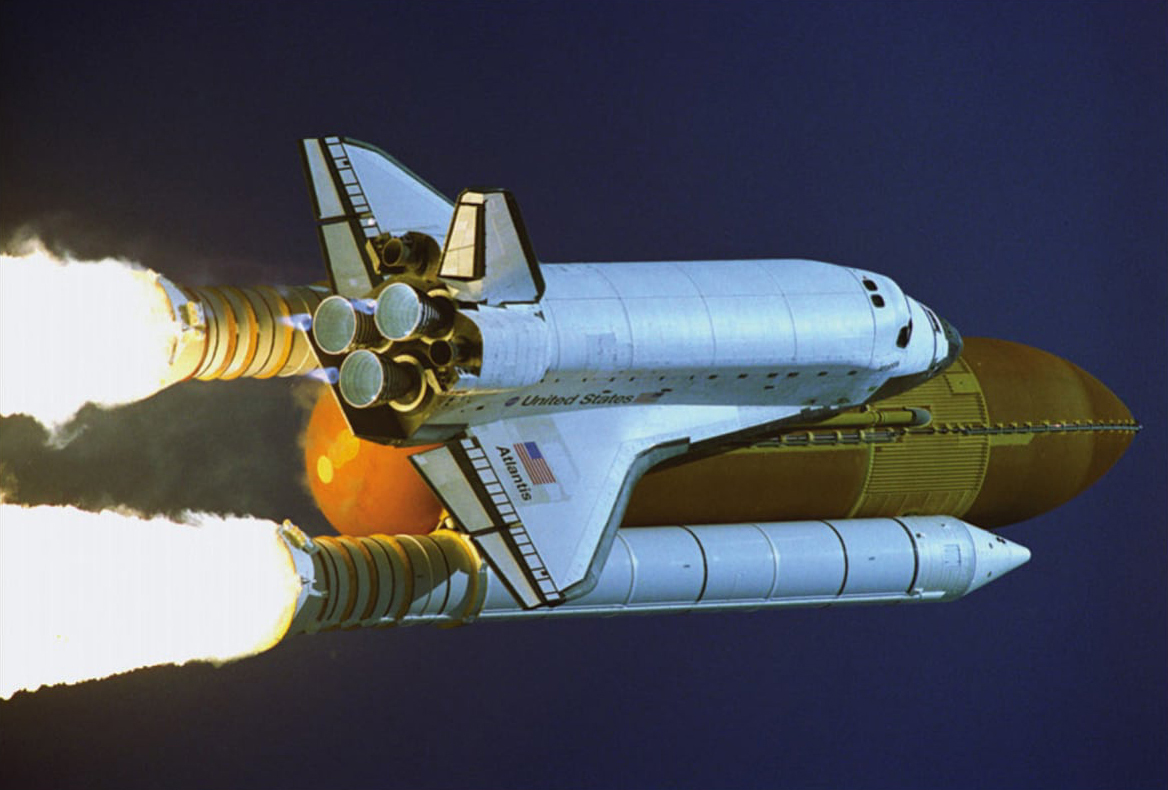
\includegraphics[width=.4\textwidth]{shuttleWithSRB.jpg}
      \end{center}
      The solid rocket boosters are the white rockets that are currently firing.
    \item With all this happening to the solid rocket boosters, they
      are surely do not have a circular cross section after all of
      this.
    \item Geometry Georigio's technique sounds good. Let's put it to the test!
      \begin{enumerate}
      \item For this one, it looks like a circle and I found three
        diameters, separated by $60^\circ$
        \begin{center}
          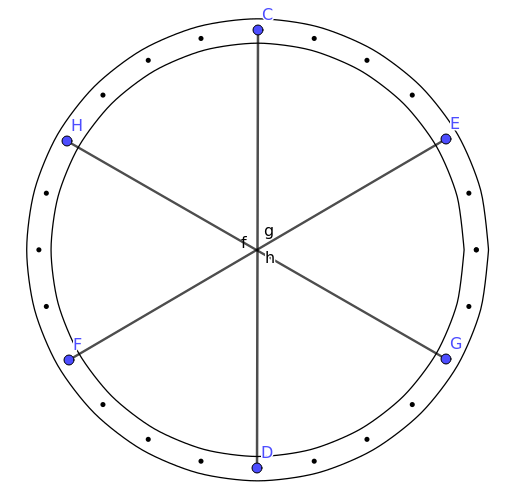
\includegraphics[width=.4\textwidth]{circleGGMeasured.png}
        \end{center}
        of measurements
        \[
        8.76,\quad 8.74,\quad 8.74.
        \]
        These are all about $8.75$, so this looks good.

      \item For this one, it looks like an oval and I found three
        diameters, separated by $60^\circ$
        \begin{center}
          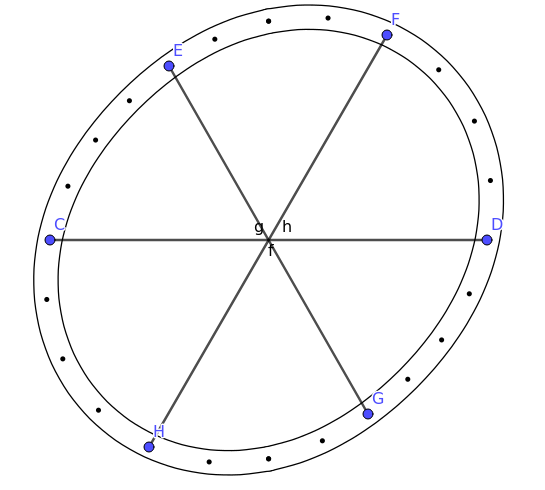
\includegraphics[width=.4\textwidth]{ovalGGMeasured.png}
        \end{center}
        of measurements
        \[
        8.74,\quad 9.52,\quad 8.02.
        \]
        These are all different, and this is not a circle, so this
        looks good too.

      \item For this one, it looks like a heart and I found three
        diameters, separated by $60^\circ$
        \begin{center}
          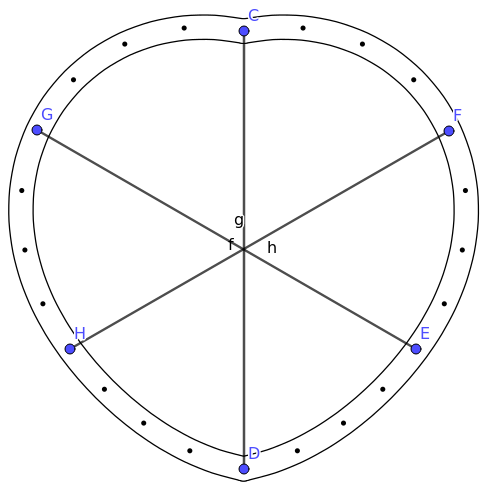
\includegraphics[width=.4\textwidth]{heartGGMeasured.png}
        \end{center}
        of measurements
        \[
        8.76,\quad 8.75,\quad 8.74.
        \]
        These are all nearly the same as a circle, BUT this is not a
        circle, so \textit{Geometry Giorgio} is WRONG.

      \item Answers may vary. A fine solution is to simply measure the
        radius, but then you need to define a ``center'' of the
        cross-section.

        Another solution, would be to think of the circular
        cross-section as being the circumcircle for a given (known)
        triangle.

        Both of these methods are better than \textit{Geometry
          Giorgio's} because they correctly identify (iii) above as
        NOT a circle.
        
      \end{enumerate}

      %% note initial screenshot at 48.2% in pdf
    \end{enumerate}
  \end{freeResponse}
\end{question}

\end{document}
